\addtocontents{toc}{\protect\newpage}
\chapter{Modelling and Statistical Analysis}
\label{sec:model}

% Why simulation.

Although first field tests and large-scale fleet trials aiming to develop recommendations for effective standardisation and charging management of electric vehicles have already been conducted e.g.\ in the projects CROME, iZeus, MeRegio in Germany \cite{Schauble2017}, the effort of testing experimental control and optimisation routines in physical systems is prohibitive; not least, because it includes interdisciplinary domains ranging from wholesale market participation to distribution network operation. Hence, it is common to turn to simulation to prove the resonance of novel optimisation approaches under varying market and network conditions.

A simulation is a valuable tool in domains, where real-world experiments are prohibitively costly, difficult to observe, or dangerous for technical equipment. It aims and succeeds at developing a better understanding of the problem at hand by replicating stylised patterns from real-world observations minted with the application of strategic behaviour on predicted parameters. Thereby, it can isolate the analysed problem from second-tier external influences.

The setting and scope of the developed simulation are pitched in \Autoref{sec:ssa}, while subsequent \Autoref{sec:sf} guides through the framework, the simulation study is implemented in. The meaningfulness of results obtained from any simulation highly depends on the quality of its inputs. Therefore, the models of individual input parameters are carefully introduced: \Autoref{sec:nt} gives an account of the used low-voltage test distribution network, while \Autoref{sec:rd} explains the generation and preprocessing of synthetic residential electricity demand profiles as well as its uncertainty representation. \Autoref{sec:ev} describes the choice of technical vehicle specification and provides an overview of possible charging system configurations. \Autoref{sec:tp} constitutes an essential part of modelling the uncertainty involved in EV charging coordination. Other than previous work it does not rely on historical data, but operates with continuous distribution fits for a user's expected average characteristics as well as typical deviation from this average, and is an addition to the research area. Ultimately, \Autoref{sec:ep} concludes the model with a representation of an adapted spot market for power trading.

\section{Setting and Scope of Analysis}
\label{sec:ssa}

Naturally, the scope of a simulation study mimicking complex systems is limited by its implementation and conjectures. To facilitate the classification of the presented study into related work on EV charging coordination, major assumptions and boundaries are summarised in the following bullet points:

\begin{itemize}
	\item Charging is exclusive to periods between the end of the last trip of the day and start of the first trip of the next day. 
	\item Charging occurs overnight at home, not at work. A particular focus lies on suburban low-voltage distribution networks without industrial loads.
	\item The penetration of electric vehicles in the network is 100\%. Of the 55 households considered, each has one electric vehicle.
	\item Charging control of private electric vehicles is devised to one central aggregator. Inter-aggregator communication and influences on the transmission system are omitted.
	\item The aggregator commands a sufficient number of electric vehicle to participate on a intra-day wholesale electricity market, but schedule day-ahead for coordination purposes. Other than day-ahead market participation, this keeps the option for instantaneous or repeated schedule adaptation in reaction to forecast deviations open.
	\item The aggregator schedules according to a charging cost minimisation problem under user satisfaction and technical constraints. It abstracts from the provision of ancillary services through discharging and is restricted to load shifting services only.
	\item Optimisation is performed on discrete time steps with a 15 minute resolution. Thereby, the actual control of network elements (e.g.\ OLTCs) and actual load and renewable generation intermittency is neglected.
	\item The optimisation horizon is 24 hours and optimisation is triggered daily at 1 pm. This time corresponds to the lowest availability probabilities of electric vehicles.
	\item Consequently, each vehicle entails 96 decision variables for each time slot within 24 hours, which represent continuous charging powers, constant within each time slot.
	\item Models and uncertainties in electricity price, residential electricity demand, EV availability, and daily distance travelled are represented by continuous distribution functions. In reality, this idealised representation would be substituted by more accurate information based on empirical behaviour logs of one specific customer and enquiries by user interfaces.
\end{itemize}

More detailed model assumptions designs are provided in the respective subsequent sections.

\section{Simulation Framework}
\label{sec:sf}

% Target

As outlined previously, consideration of uncertainties about EV scenarios is more prevalent in related work than the recognition of individual uncertainties in mobility patterns \cite{Soares2011, Dallinger2010a}, residential demand and market prices. The composed simulation framework seeks to unite both aspects: it comprises Monte Carlo analysis to cope with scenario uncertainty regarding the allocation of consumer types and general market conditions, while it also addresses the second-tier operational uncertainties.

% optimisation routine

The routine of the simulation study is structured as shown in \Autoref{fig:optroutine}:  After retrieving general parameters such as optimisation horizon, resolution of discrete time steps, starting time index, algorithm choice and parameters, the scenario is stochastically generated comprising behavioural as well as market models. In consequence, scenarios describe the model parameters of imaginable nights in which vehicles are scheduled on the same test network. It is important to note that a scenario refers to the allocation of e.g.\ certain user \textit{characteristics} in the network but not to the \textit{realisation} of uncertainties defined by the user type. Should information about voltages and line loadings in the distribution network be approximated by linear power flow, corresponding network sensitivities are determined beforehand and will be valid for all scenarios based on the same test network.

\begin{figure}[tp]
	\includegraphics[width=\textwidth,trim={0.5cm 0.5cm 0.5cm 0.5cm},clip]{figures/framework/optimisationroutine}
	\caption{Flow Chart of Optimisation Routine in Simulation Framework}
	\label{fig:optroutine}
\end{figure}

The assessment of a scheduling approach for a specific scenario is based on three stages: the \textit{optimisation} schedules and coordinates EV charging processes according to the selected problem formulation, algorithm, and uncertainty mitigation options based on the forecasted parameters. Subsequently, the \textit{simulation} realises deviations from these forecasts in accordance with their uncertainty models and determines performance measures such as charging costs, fulfilment of customer demands, and observation of network constraints of the original optimised schedule. To compare these results to the optimal schedule that could have been achieved with the same algorithm had all the parameters been known \textit{ex ante}, the  \textit{benchmark} stage applies the selected algorithm with perfect information. In conjunction with the simulation results, the robustness of the optimisation algorithm to uncertainty can be assessed.

% Monte Carlo

Different optimisation algorithms and reference cases are evaluated relative to each other by running the same framework with identical parameter sequences. Because performance analysis of algorithms in a single scenario is inexpressive, the optimisation routine is coupled with a Monte Carlo (MC) simulation as applied in \cite{Navarro2013a, Navarro2013}. Arbitrary circumstances may favour one algorithm over another and, thereby, warp the evaluation. To hedge against this randomness, a series of scenarios are generated stochastically forming the basis of comparative performance assessment. Due to the multitude of scenarios optimised, a more accurate evaluation through distributions of performance measures is attained. Note that here the Monte Carlo simulation wraps the optimisation cycle and is not a component within the optimisation routine as used in e.g.\ \cite{Sandels2010}. Applied optimisation algorithms are exclusively deterministic. The many stochastic input parameters are entered either with their true expectation values or adapted through more conservative estimates.

% software architecture

The simulation framework has been implemented with an object-oriented approach in Python interfaced with the open source simulation tool OpenDSS to enable fast power flow (PF) studies of electrical distribution systems \cite{Ochoa2015}. OpenDSS origins from work by the Electric Power Research Institute and facilitates script-driven serial power flow simulations throughout a day in addition to snapshot analyses, pivotal to the impact evaluation of electric vehicle scheduling. Moreover, a series of IEEE test feeders are readily implemented in OpenDSS. It runs a three-phase unbalanced load flow using input data defined in \Autoref{sec:nt}.

\section{Network Topology}
\label{sec:nt}

Among the provided test distribution networks, the IEEE European Low Voltage Test Feeder developed in OpenDSS has been selected \cite{unknown2015}. Some studies focus on mitigating aggregated EV impacts in MV distribution networks \cite{Galus2011,GonzalezVaya2015a,Schwerdfeger2012}, but heavily loaded LV European distribution networks are likewise prone to technical issues caused by a market uptake of electric vehicles \cite{Quiros-Tortos2016}. Other than MV distribution networks, LV networks were traditionally designed with a \textit{fit and forget} attitude with little attention paid towards monitoring and operations management beyond power flows from the substation transformer. The penetration of low-carbon technologies demand a more active management approach towards low-voltage distribution circuits to avoid excessive voltage deviations, the transgression of thermal line limits, and phase unbalances of electric loads \cite{Ochoa2012}.

Many of the IEEE test cases are focused on North American 120/240 V single-phase distribution networks. Typically, these are characterised by an extensive MV system and a simple LV network, where there are only a handful of households connected to one transformer. However, European networks differ significantly as they consist of much simpler MV networks and more complex LV network structures \cite{Heinrich2012}. Fewer MV/LV transformers connect many more households via 230/400 V three-phase cables. Radial and meshed layouts are the two principal types of distribution grids. Meshed networks are prevalent in urban areas and possess multiple connections to the MV grid with interlinked feeders to hedge against the risk of outages due to maintenance operations or faults \cite{Ochoa2012}. Radial networks are more typical of rural and suburban areas. Their tree-shaped layout with a central connection to the MV network branching towards individual households is characteristic of the IEEE European Low Voltage Test Feeder. Therefore, the study will focus on suburban European distribution networks and resembles distribution networks modelled in related works \cite{Melhorn2017, Navarro-Espinosa2014, OConnell2014, Connell2012, Quiros-Tortos2016, Richardson2012a}. 

The radial distribution feeder operates at a line-to-line voltage of 400 V and a base frequency of 50 Hz. It is connected to the MV system through an 11/0.4 kV transformer at one central substation. The three-phase transformer is generously rated at 0.8 MVA with a delta/grounded-wye connection and does not provide any tap-changing capability. The MV network is modelled as an 11 kV voltage source with an impedance specified by three-phase and single-phase short circuit currents at 3 kA each. The main feeder and laterals amount to 905 three-phase lines connecting 906 buses, whose characteristics are defined by line codes including sequence impedances and admittances and lengths. Because the test feeder originally does not provide values for line ampacities, these have been acquired from a LV capacitor placement study by Electricity North West \cite{ENWL2013}. 

\begin{figure}[tp]
	\includegraphics[width=\textwidth,trim={0cm 0cm 0cm 0cm}, clip]{figures/network/network_layout.pdf}
	\caption{Network topology and load locations of IEEE European low voltage test feeder}
	\label{fig:network}
\end{figure}

A geographical single-line diagram of the network is depicted in \Autoref{fig:network}. The test network comprises 55 numbered households connected to a single phase. The loads are rather evenly spread across the phases with 20 homes connected to each, phase 1 and phase 2, and 15 households attributed to phase 3. For simplicity, no further loads by industrial customers nor local photovoltaic generation are considered in the network.

% \cite{Bohn2017} 

\section{Residential Demand}
\label{sec:rd}

% Why?
Evaluating the functionality and impact of EV scheduling schemes in the low-voltage distribution network requires not only knowledge of EV loads but also a detailed insight into the spatial and temporal occurrence of residential loads. Considering high-resolution demand profiles that represent the variability of individual demands enables a comprehensive modelling of the network state and sensitivities to additional EV loads \cite{McKenna2016}. 

\subsection{Modelling}
% Generation of pool
A pool of 1000 individual residential electricity demand profiles, from which the stochastic scenario generation can choose, was created with the commonly used CREST demand model developed at Loughborough University \cite{Richardson2011}. Taking into account multiple factors such as the type of day, season, geographical location, and the number of occupants, it builds synthetic residential loads from individual devices and consumption activities. Consumer behaviour is modelled by Markov chains whose transition probabilities are derived from time-use surveys \cite{Richardson2010a,Richardson2008}. The output is a realistic 1-min resolution profile for domestic electricity demand of UK customers. 

To capture the sensitivity of residential loads to the number of active inhabitants in a household, the 1000 profiles were generated considering the proportion of homes with a given number of residents in the UK \cite{Figueiredo2005}. Households with one, two, three, four and five inhabitants are represented with 34\%, 40\%, 14\%, 9\% and 3\% respectively. More detailed clustering for load forecasts has been undertaken but is omitted for the sake of exposition \cite{Wu2007,Sousa2009}.

% Assumptions
Each household in the test network was assumed to maintain a constant inductive power factor of 0.96. For simplicity, no seasonal electricity demand variation is considered. Without loss of generality, the load profiles are confined to typical weekdays during winter capturing maximum demand in the UK. Furthermore, while some constituents of the residential demand might be deferrable and could be used for demand-side management, they are considered to remain static loads. 

% Assignment
For the stochastic scenario generation, electricity demand profiles were randomly assigned to each single-phase customer in the test distribution network. As the optimisation starts midday but the stored patterns are ordered from 0:00 am to 11:59 pm, the profiles are shifted by their difference of start indices. The adopted profiles are then resampled to match the chosen resolution of the optimisation routine. It is important to note that reducing the resolution will underestimate the temporal variability and, thereby, spoil the representation of instantaneous demand peaks as illustrated by three exemplary individual demand profiles for varying resolutions in \Autoref{fig:ind15min}, \Autoref{fig:ind5min} and \Autoref{fig:ind1min}.

\begin{figure*}[tp]
	\centering
	\begin{subfloat}
		\centering
		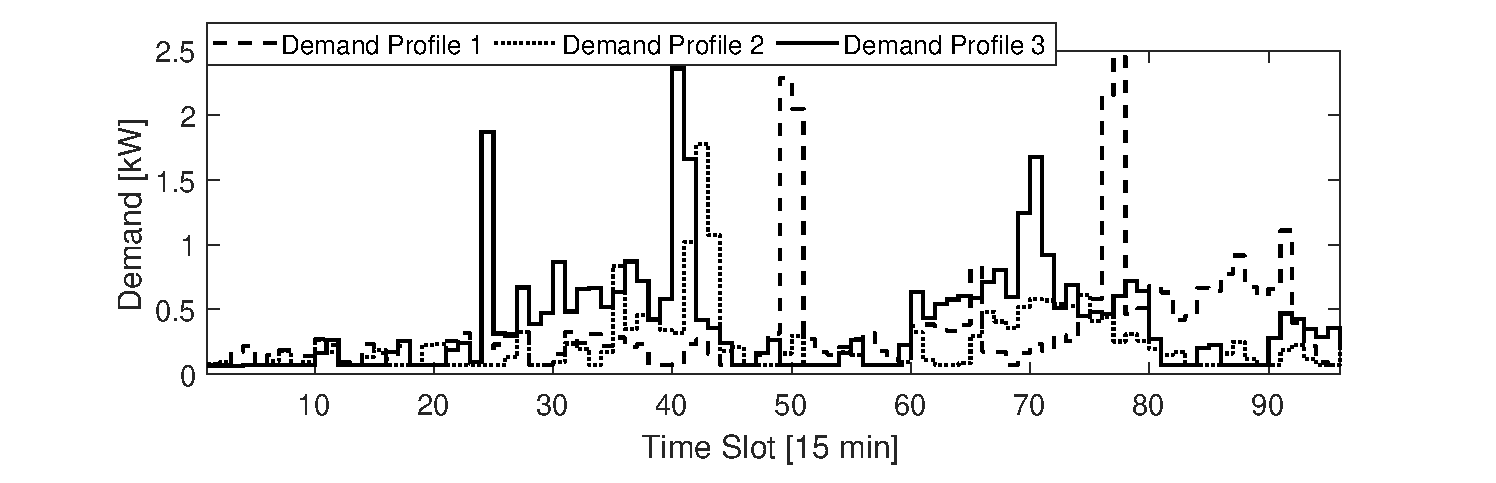
\includegraphics[width=.76\textwidth,trim={3cm 0cm 3cm 0cm}]{figures/demand/15minind.eps}
		\caption{Exemplary residential demand profiles 15-min resolution}
		\label{fig:ind15min}
	\end{subfloat}%
	\begin{subfloat}
		\centering
		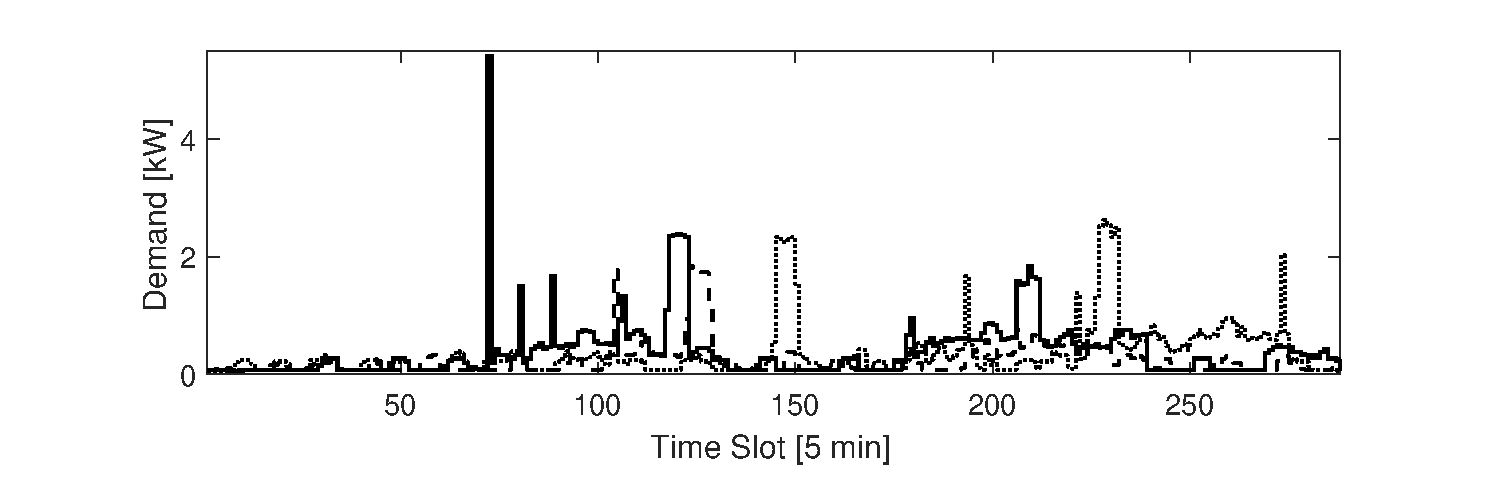
\includegraphics[width=.76\textwidth,trim={3cm 0cm 3cm 0cm}]{figures/demand/5minind.eps}
		\caption{Exemplary residential demand profiles 5-min resolution}
		\label{fig:ind5min}
	\end{subfloat}
	\begin{subfloat}
		\centering
		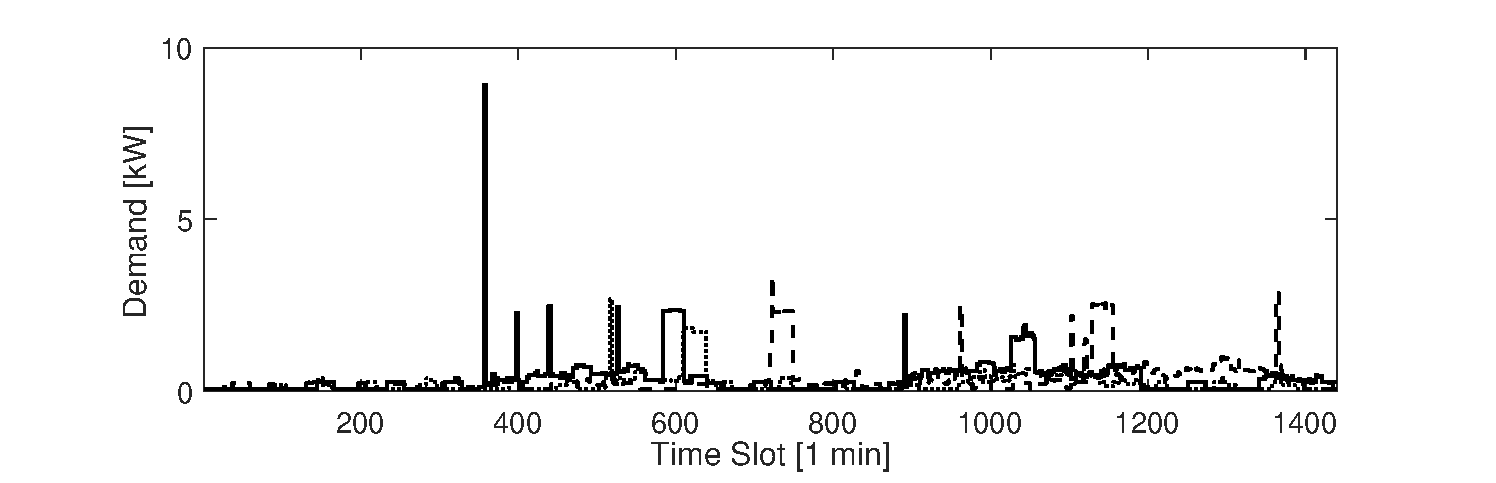
\includegraphics[width=.76\textwidth,trim={3cm 0cm 3cm 0cm}]{figures/demand/1minind.eps}
		\caption{Exemplary residential demand profiles 1-min resolution}
		\label{fig:ind1min}
	\end{subfloat}
\end{figure*}

% Figures
\Autoref{fig:demandboxplots} depicts the distribution spread of loads at each time slot via box plots highlighting both temporal correlation and the diversity of the time series. Aggregating all stored synthetic demand profiles and a comparison with the normalised ELEXON standard load profile \cite{ELEXON2017} for unrestricted domestic customers as shown in \Autoref{fig:aggregatedemandd}, confirms the approximate validity of the pool of load profiles.

\begin{figure}[tp]
	\centering
	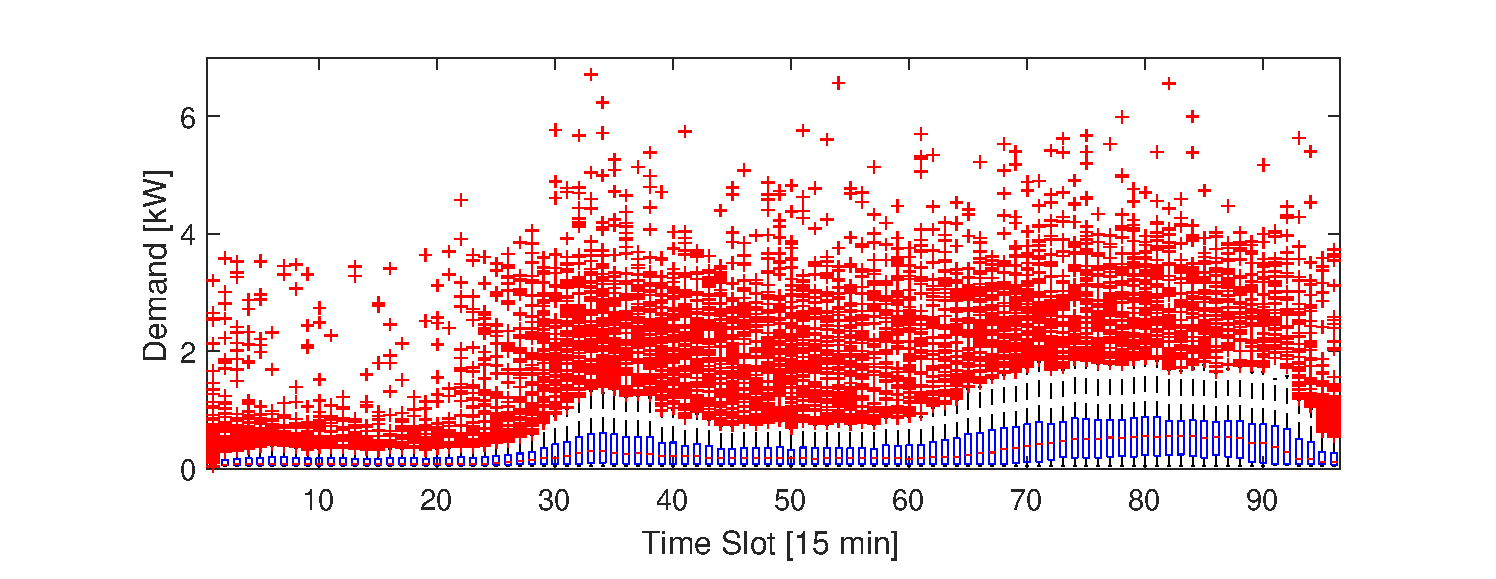
\includegraphics[width=.9\textwidth,trim={2cm 0cm 2cm 0cm}, clip]{figures/demand/indbox.eps}
	\caption{Boxplots of individual electricity demands}
	\label{fig:demandboxplots}
\end{figure}

\begin{figure}[tp]
	\centering
	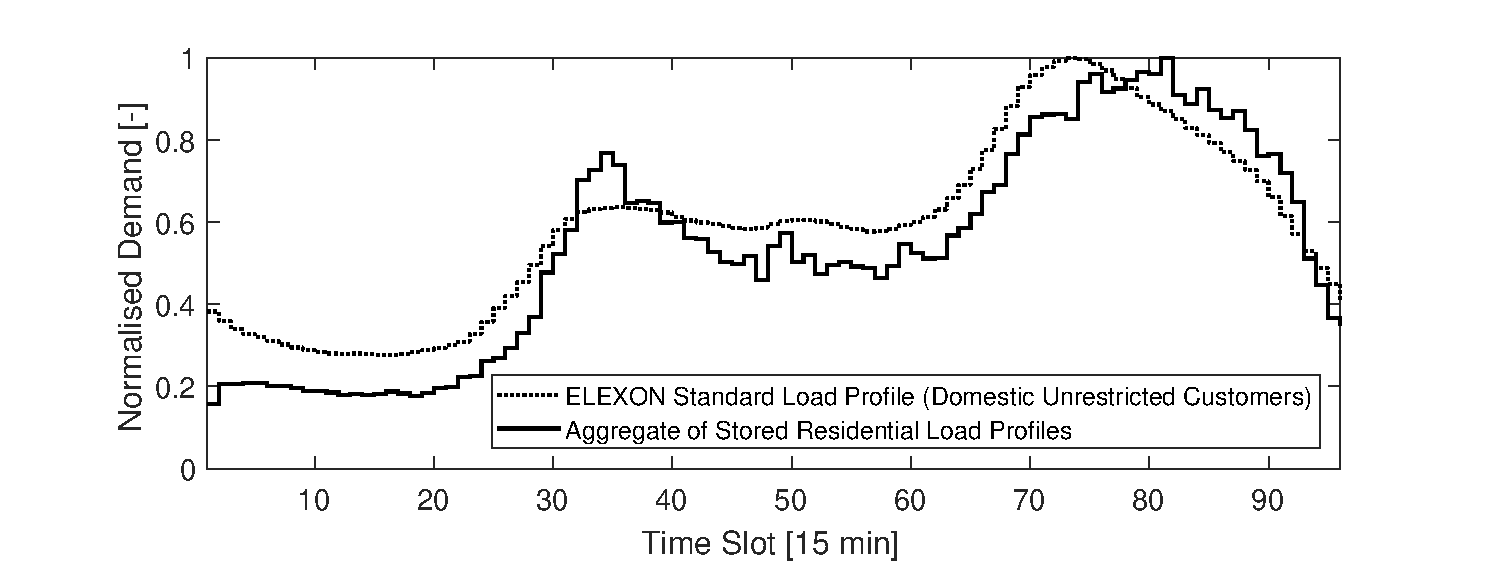
\includegraphics[width=.9\textwidth,trim={1.5cm 0cm 2cm 0cm}, clip]{figures/demand/aggdemand.eps}
	\caption{Aggregate electricity demand of stored profiles versus ELEXON average load profile}
	\label{fig:aggregatedemandd}
\end{figure}

\subsection{Uncertainty Representation}
\label{sec:rd_unc}

% Uncertainty
While on an aggregate scale consumer behaviour is quite accurately predictable, predicting individual behaviour is prone to substantial inaccuracies despite elaborate forecasting techniques \cite{Bandyopadhyay2015,Nguyen2015,Gajowniczek2017,Sevlian2014a,Riaz2007}. Multiple dimensions of uncertainty may be considered in terms of residential electricity demand; namely \textit{whether}, \textit{when}, and \textit{what amount} of electricity is required at an individual households. 

With smart metering infrastructure at the household level becoming increasingly available, more insight is obtained about the \textit{amount} of powers required in certain time frames \cite{Flath2012,Figueiredo2005}. While the exact time of an activity with a particular power demand heavily depends on customer behaviour, the prediction of the magnitude of this activity is less insecure. Most significant appliances are used on a regular basis and exhibit characteristic power signatures. Hence, deviations of simulated power demand magnitudes from their predictions are neglected.

Moreover, the uncertainty \textit{whether} a characteristic load is a second-tier problem. First, if the conservative default assumption is that an appliance is used, then unexpectedly not using this device will rarely lead to voltage or line loading problems in a heavily loaded distribution network and only marginally block network capacity for EV loads. Second, many typical cases where appliances are not used against typical behaviour -- such as holidays -- may be queried by a user interface releasing additional network capacity for EV loads.

Consequently, the uncertainty representation of residential electricity demand concentrates on \textit{when} characteristic household-level demand peaks occur. Although the deviations in the timing of different characteristic demand peaks throughout the day are likely to be independent, for simplicity they are modelled to be perfectly correlated. Thereby, the uncertainty of the demand forecast can be represented by shifting the simulated time series by a random duration. Let $w$ be the realisation of the random variable $W\sim \mathcal{U}(-w_{max},w_{max})$ denoting the uniformly distributed temporal deviation of the demand forecast $\hat{D}_t$ from the simulated demand $D_t$ within the maximum deviation $w_{max}=0.5$ h. Then the relation of predicted and simulated demand is given by

\begin{equation}
\hat{D}_t = D_{(t+w)\;\text{mod}\; T} \qquad \forall t\in T
\end{equation}

where the modulo operator assures that a continuous rolling maximum can be provided for the margins of the optimisation horizon.

\section{Electric Vehicles}
\label{sec:ev}

\subsection{Technical Vehicle Specifications}

\begin{table}[tp]
	\centering
	
	\begin{tabular}{@{}lllll@{}}
		\toprule
		\textbf{Vehicle Model}               & \textbf{Curb Weight}    & \textbf{Range}           & \textbf{Battery Capacity} & \textbf{Consumption}    \\ 
		& {[}kg{]}       & {[}km{]}        & {[}kWh{]}        & {[}kWh/km{]}   \\ \midrule
		Citro�n C-Zero              & 1,110          & 150             & 16               & 0.107          \\
		Karabag Fiat 500 E          & 2,340          & 130             & 28               & 0.215          \\
		Ford Transit Electric       & 1,120          & 140             & 20               & 0.148          \\
		Mercedes A-Class E-Cell     & 1,591          & 255             & 36               & 0.141          \\
		Nissan Leaf                 & 1,520          & 160             & 24               & 0.15           \\
		Peugeot iOn                 & 1,110          & 150             & 16               & 0.107          \\
		Renault Fluence Z.E.        & 1,610          & 185             & 22               & 0.119          \\
		Renault Kangoo Z.E.         & 1,410          & 170             & 22               & 0.129          \\
		Renault Zoe                 & 1,392          & 210             & 22               & 0.105          \\
		Smart Fortwo Electric Drive & 975            & 140             & 18             & 0.126          \\
		Tesla Roadster              & 1,220          & 393             & 53               & 0.135          \\
		Think Global Th!nk City     & 1,038          & 160             & 23               & 0.144          \\
		Tesla Modell S              & 2,108          & 335             & 60               & 0.179          \\
		Toyota RAV 4 EV             & 1,830          & 160             & 42               & 0.261          \\
		BMW i3                      & 1,315          & 183             & 33               & 0.169          \\ \midrule
		\textit{Average}            & \textit{1,446} & \textit{194.73} & \textit{29.01}   & \textit{0.150} \\ \bottomrule
	\end{tabular}
	\caption{Technical data of selected currently marketed electric vehicles \cite{Schuller2013,Salah2012,DepOfTrans2017} }
	\label{tab:evspec}
\end{table}

The relevant characteristics for modelling EV loads are the consumption rate, battery capacity and maximum range. A survey of the currently marketed electric vehicle produced the compilation of EV specifications in \Autoref{tab:evspec}. The list includes the top fully electric models of ultra-low emission vehicles (ULEV) registered for the first time in the UK in 2016 and commonly used reference vehicles in the literature \cite{DepOfTrans2017}. Noting a recent trend of increasing battery size and electricity consumption, the model assumes a single consumption rate of $\zeta=0.17$ kWh/km and a capacity of $B_{max}=30$ kWh for all modelled electric vehicles. Thereby, the consumption rate $\zeta$ creates a direct correspondence between battery capacity and vehicle range, although in reality using a singular value is a simplification; the amount of energy that an electric car consumes depends on a number of external factors such as the ambient temperature, driving speed, and the height profile of the covered track. Furthermore, neither battery degradation nor losses from storing electricity are considered in the technical EV model.

\subsection{Charging System Specification}

Details on charging infrastructure for the grid connection of electric vehicles encompass two major aspects: the physical network connection as well as communication and control ability. A multitude of connector types and charging modes exist differing in voltage and current levels, the number of phases or the type of connectors used. Which specifications prevail is largely dependent on the historical developments and traditions of both, distribution network operators and vehicle manufacturers \cite{Bossche2010}. Particular differences in specifications, as well as terminology, are noted between the USA and European countries. Regardless of location, conductive charging methods using cables and plugs can be distinguished from inductive methods transferring power magnetically. The former is current standard for EV grid connection and, thus, at the focus of subsequent analysis. Charging \textit{modes} summarise standards of connection specifications and infrastructure requirements, whereas charging \textit{levels} give a broader notion of power ranges with charging levels 1, 2, and 3 used in the context of US power systems and their European equivalents standard, semi-fast, and fast. An overview of charging modes, levels, plugs and their specifications is provided in \Autoref{tab:chargingmods}.

% Please add the following required packages to your document preamble:
% \usepackage{booktabs}
% \usepackage{multirow}
\begin{table}[tp]
	\centering
	\resizebox{\textwidth}{!} {%
	\begin{tabular}{@{}lllllll@{}}
		\toprule
		\textbf{Charging}          & \textbf{Charging} & \textbf{Charging}  & \textbf{Phases}  & \textbf{Voltage} & \textbf{Current} & \textbf{Power}    \\ 
		\textbf{Mode}              & \textbf{Levels}   & \textbf{Plug}      & \textbf{{[}-{]}} & \textbf{{[}V{]}} & \textbf{{[}A{]}} & \textbf{{[}kW{]}} \\ \midrule
		\multirow{5}{*}{Mode 1, 3} & EU Standard       & CEE7 / Type 2      & 1                & 230              & 16               & 3.7               \\
		& EU Semi-Fast      & Type 2             & 1                & 230              & 32               & 7.4               \\
		& EU Semi-Fast      & Type 2             & 3                & 400              & 16               & 11.1              \\
		& EU Semi-Fast      & Type 2             & 3                & 400              & 32               & 22.2              \\
		& EU Fast           & Type 2             & 3                & 400              & 63               & 43.6              \\ \midrule
		Mode 1, 2                  & US Level 1        & Nema 5-20 / Type 1 & 1                & 120              & 15               & 1.8               \\
		Mode 2, 3                  & US Level 2        & Type 1             & 1                & 240              & 30               & 7.2               \\ \midrule
		\multirow{2}{*}{Mode 4}    & US Level 3 DC     & Type 4 / CHAdeMO   & -                & 50-500           & 100              & 50                \\
		& EU Fast DC        & Type 2 Combo       & -                & 500              & 140-200          & 70-100            \\ \bottomrule
	\end{tabular}
	}
	\caption{Charging modes, levels, plugs and their specifications for $\cos\phi=1$ (adapted \cite{Bossche2010, Yilmaz2012, Schuller2013})}
	\label{tab:chargingmods}
\end{table} 

\textbf{Mode 1} refers to the direct connection of electric vehicles to AC networks with standard socket outlets, which do not exceed 16 A. Despite comparably low power levels, it can provide adequate energy for overnight charging. Mode 1 uses non-dedicated infrastructure for private premises that is readily available, which makes it the cheapest and most common approach. However, mode 1 does not employ protective equipment, particularly for EVs nurturing safety concerns. The sole protective elements used are a fuse or circuit breaker against overcurrents, earthing connection and, depending on the age of a building, residual current devices (RCD) to avoid detrimental leakage currents. 

\textbf{Mode 2} also uses standardised sockets but adds further protection via a control box with a control pilot conductor between vehicle and plug \cite{Bossche2010}. Although it remedies some safety concerns, it is restricted to cable protection and disregards the plug itself which may be more liable to damages during operation. Moreover, no communication protocols for control purposes are enabled.

\textbf{Mode 3} defines the direct grid connection of electric vehicles to the AC network utilising dedicated EV supply equipment \cite{Schuller2013}. According to the IEC Standard 61851-1, it mandates control pilot protection applied to enable continuous control and charge rate modulation. Its roles are summarised in \cite{Bossche2010} in four categories as

\begin{itemize}
	\item verification that the vehicle is properly connected,
	\item continuous verification of the protective earth conductor integrity,
	\item energisation and de-energisation of the system, and
	\item selection of charging rates.
\end{itemize}

While originally the IEC Standard 61851-1 demanded an additional conductor to phase(s), neutral and earth as control pilot, an update opened the standard for other means to provide this functionality. Classically, the variation of charge rate was realised through a change of the duty cycle of a pulse-width modulation (PWM) signal to convey information about the desired charging power. Mode 3 allows varying degrees of communication with other entities, ranging from no communication for mere safety purposes to intense information exchange for identification, billing, and devised charging control. Communication protocols are currently defined by standards ISO TC22 SC3, ISO TC22 SC21, and IEC TC 69.

\textbf{Mode 4} refers to the indirect grid connection of electric vehicles using off-board chargers with a communication link to the EV battery. It is most relevant for DC charging systems with high charging powers. It must be noted that mode 4 is restricted to public charging stations for it exceeds the maximum power level of EU residential connections with standard outlets of \mbox{11.1 kW}.

Taking the characteristics and costs of different charging modes and levels into account, the built model focusses on single-phase mode 3 charging following European distribution network characteristics. This is a compromise between individual investment costs for charging infrastructure resulting in acceptance barriers and the capability of information exchange and charge rate modulation. Moreover it fits well with the approach to utilise EV load flexibility in residential distribution networks overnight at single-phase connected households.

Although concepts of bidirectional power flow to and from EV batteries exist, such vehicle-to-grid (V2G) capability is disregarded in the model. While this would free up more flexibility for the provision of ancillary services, spinning reserves, reactive power support, peak shaving and energy balance services, in essence, these services may also be provided by unidirectional control. It is only expected to become available for semi-fast charging levels and require high investment costs. Moreover, it would likely add to battery degradation due to more frequent cycling and may require adapting the distribution system \cite{Yilmaz2012}.

A comprehensive technical overview of infrastructure requirements is provided in \cite{Yilmaz2012}. Although the internal resistance of EV batteries is low, the charging process is not lossless. Hence, the model assumes a constant charging efficiency of $\eta = 0.93$, following the work of \cite{Flath2013}. This abstracts from the quadratic loss scaling at increasing charging currents, whose impact has been reported limited for capacity normalised charging rates between 0.1 and 1.0 \cite{Flath2013}. The preceding discussion results in an EV model with the parameters displayed in \Autoref{tab:evmodel}.

% Please add the following required packages to your document preamble:
% \usepackage{booktabs}
\begin{table}[tp]
	\centering

	\begin{tabular}{@{}llll@{}}
		\toprule
		\textbf{Parameter}                    & \textbf{Symbol}                   & \textbf{Values} & \textbf{Unit} \\ \midrule
		Battery capacity                      & $B_{max}$                         & 30              & kWh           \\
		Consumption rate                      & $\zeta$                           & 0.17            & kWh/km        \\
		Maximum charge rate                   & $P_{max}$                         & 3.7		        & kW            \\
		Minimum charge rate                   & $P_{min}$                         & 0.0             & kW            \\
		Charging efficiency                   & $\eta$                            & 0.93            & -             \\
		Maximum charge amount per slot        & $\eta\cdot\Delta t\cdot P_{max}$  & 0.860           & kWh           \\ 
		Maximum charging power rate of change & $\Delta_{max}$                    & \{0.925,3.7\}   & kW            \\ \bottomrule
	\end{tabular}
	\caption{Summary of electric vehicle model parameters}
	\label{tab:evmodel}
\end{table}

\section{Travel Patterns}
\label{sec:tp}

Besides technical vehicle specifications, appropriate behaviour models of the daily travel patterns are essential for the analysis of efficient charging coordination. Consequently, a model of the general driving habits of individual EV owners completes the EV model primitives. The overall process is depicted in \Autoref{fig:flow} and explained in detail in following subsections.

\begin{figure}[]
	\centering
	\includegraphics[width=.9\textwidth,trim={0cm 0.5cm 0cm 0.8cm},clip]{figures/mobility/flow}
	\caption{Illustration of travel pattern model derivation and application}
	\label{fig:flow}
\end{figure}

\subsection{Data Source and Extraction}

% mention possible data sources and assumptions made

Due to the limited market penetration of electric vehicles to date, appropriate data sets on the mobility of EV owners are sparse. To circumvent this problem, the developed model is based on empirical driving profiles of internal combustion vehicles. Thereby, it is assumed that a majority of travel patterns will not be influenced by a transition from conventional vehicles to electric vehicles in private transport, although this is not unquestioned \cite{Schauble2017}. Nonetheless, this approach is commonly applied in research on EV charging modelling and is deemed particularly reasonable for inferring charging requirements \cite{Schuller2013,Flath2013, Wang2017, Daina2017,Pasaoglu2013,Wu2010b}. 

To model the behaviour of UK customers, mobility data was obtained from the UK National Travel Survey \cite{NTS2017}. This extensive survey is updated annually and contains a multitude of disaggregated data about means, demographics and behaviour of personal travel based on record diaries from 2002 to 2015. Given the amount of data provided, only a sufficiently large extract of trip data of the most recent 4,000 households with a total of 30,000 trips by car logged was used. 

% simplifications regarding clustering and weekday differentiation & neglected differentiations

As trip data is quite heterogeneous regarding trip purposes, weekdays and demographic groups, clustering as undertaken in related work appears sensible and will result in a differentiated representation of the reality \cite{Schuller2013, Acha2012}. For the sake of exposition, the developed mobility model focusses on weekdays and makes no differentiation between demographic groups or trip purposes. Although this simplification lacks the sophistication achieved by clustering, it will comprise the most challenging days for EV charging and could easily be remedied by mere repetition of analysis. Hence, the trip data is filtered only to extract trips by cars on weekdays. Moreover, to avoid too small sample sizes households with less than three days logged in the record books are excluded. Subsequently, the data set was examined further to find measures for the average $\mu$ and standard deviation $\sigma$ of daily mileage, arrival and departure times of individual households. This provides an alternative to developing a stochastic mobility model based on Markov chains or agent-based methods as elaborated in i.a.\ \cite{Soares2011, Acha2012,Galus2011,Hu2016}. However, involved uncertainty has only been analysed for a limited number of studies \cite{Wang2017,Zhang2014}.

% describe method of size reduction and pre-calculations on data set 

\subsubsection*{Arrival and Departure Times}

In practice, an electric vehicle may arrive and depart at multiple locations and times of the day. But, because the assumed scenario is confined to scheduling for charging at home overnight, the ambiguity of the terms arrival and departure time can be resolved \cite{Dallinger2010a}. While the arrival time refers to arrival at home after the last trip of the day, the departure time refers to the departure from home just before the first journey of the next day. For each household, the average and standard deviation of these arrival and departure times among the logged days are determined and compiled to two sets of ($\mu$,$\sigma$)-tuples characterising the required information about a household's EV availability.

\subsubsection*{Daily Mileage}

Daily trip distances in the data set are obtained from the sum of all individual trips for each household and logged day. Given the range of modelled electric vehicles as specified through the battery capacity and consumption in \Autoref{sec:ev}, infeasible trip distances outwith the EV range of 120 miles are discarded. Then, similar to the arrival and departure times, the values for the daily mileage are recorded as a set of ($\mu$,$\sigma$)-tuples describing a car's typical driving distance.

\subsection{Analysis of Empirical Data}

% qualitatively analyse histograms of empirical data

Histograms of the acquired ($\mu$,$\sigma$)-tuples are depicted in \Autoref{fig:mobilityfits}, emphasising the heterogeneity of both average and variance values of parameters among participating households. In an average household, the first trip by car occurs at 10:30 am while the last trip ends 16:45 pm. Throughout the day this household has travelled 22 miles or 35 km. Normally, an average household deviates between 2 and 2.5 hours from its average departure/arrival times and 15 miles or 24 km from its expected daily mileage. These values are surprisingly high and exceed expectations on the uncertainty involved. A comprehensive list of shape parameters such as skewness and kurtosis are compiled in \Autoref{tab:shapeparams}.

\begin{figure}[tp]
	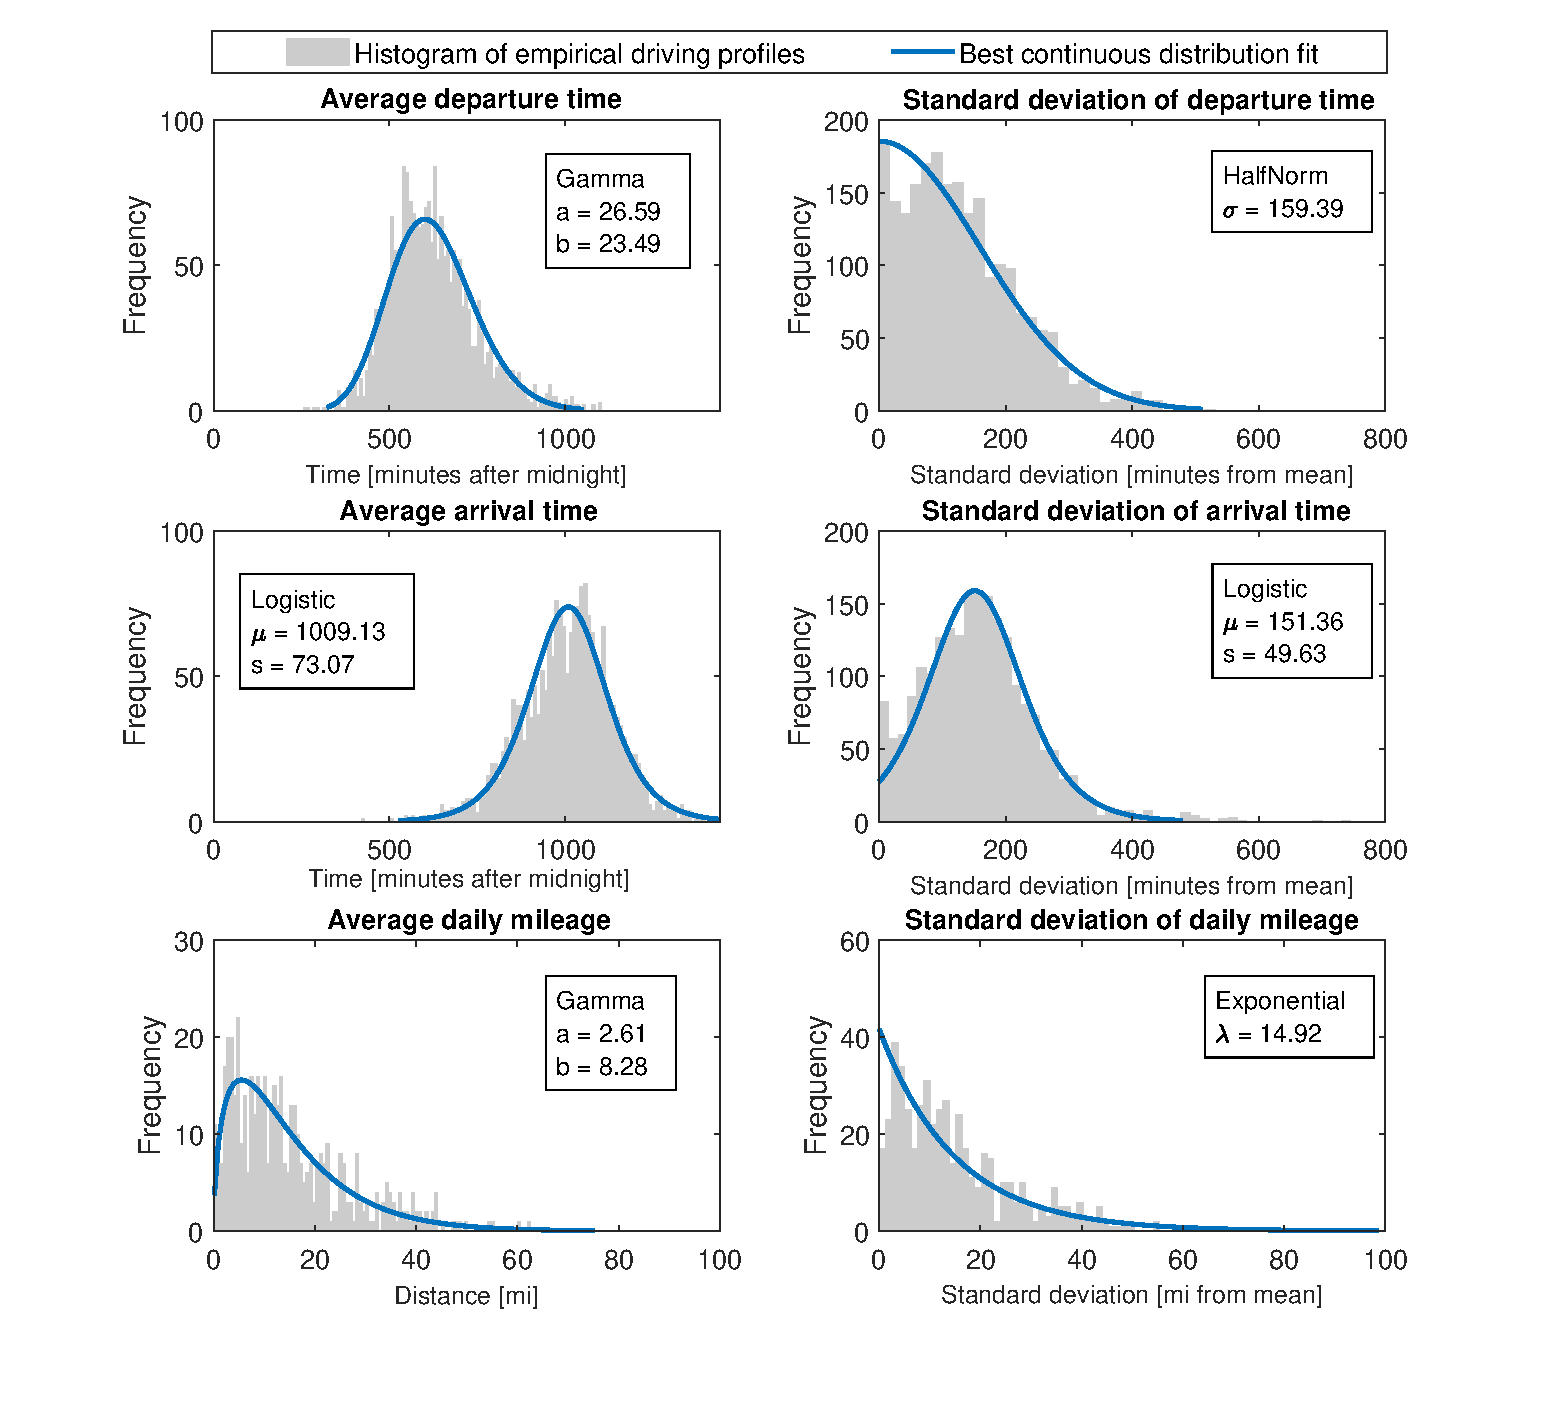
\includegraphics[width=\textwidth,trim={1.5cm 1.2cm 2cm 0cm},clip]{figures/mobility/mobilityfits.eps}
	\caption{Marginal distribution fits of ($\mu$,$\sigma$)-tuples of daily mileage, arrival and departure times}
	\label{fig:mobilityfits}
\end{figure}

% describe parameters of marginal distribution fits

\Autoref{fig:mobilityfits} moreover includes continuous distributions fitted to the empirical driving profiles. Extracting the relevant statistical information from the travel survey to build a generic EV user model without massive data sets facilitates its scalability, reproducibility and calibration. Approximating driving distances by Gamma distributions has been applied and validated in research papers \cite{Flath2013, Plotz2017}.

The distribution for each parameter is chosen based on the Akaike information criterion (AIC) which compares the relative quality of models for a given data set. This approach results in four types of distributions describing the six random variables of the mobility behaviour model, the parameters to which are complemented in \Autoref{fig:mobilityfits}.

Average departure time and daily mileage are described by a Gamma distribution denoted by the probability density function

\begin{equation}
f_{\mathrm{Gamma}}(x;a,\theta) = \begin{cases}
\frac{ \theta^{-a}}{\Gamma(a)}x^{a-1} e^{- \frac{x}{\theta}} & x \geq 0 \\
0 & x < 0
\end{cases} \quad \text{ for } a, \theta > 0
\end{equation}

The average and standard deviation of arrival times are approximated by a truncated logistic distribution with the probability density function

\begin{equation}
f_{\mathrm{Logistic}}(x; \mu,s) = \begin{cases}
\frac{e^{-\frac{x-\mu}{s}}} {s\left(1+e^{-\frac{x-\mu}{s}}\right)^2} & x \geq 0 \\
0 & x < 0
\end{cases}
\end{equation}

The standard deviation of departure times follows a half normal distribution with the probability 

\begin{equation}
f_{\mathrm{HalfNorm}}(x; \sigma) = \left|\frac{\sqrt{2}}{\sigma\sqrt{\pi}} \,\cdot\, e^{-\frac{x^2}{2\sigma^2} } \right|
\end{equation}

Finally, the standard deviation of daily mileage shows exponential characteristics with the probability density function

\begin{equation}
f_{\mathrm{Expo}}(x;\lambda) = \begin{cases}
\lambda e^{-\lambda x} & x \ge 0, \\
0 & x < 0.
\end{cases}
\end{equation}

% discuss quality and validity of marginal distribution fits

The accuracy of the fits could be confirmed neither by a Kolmogorov-Smirnov nor a $\chi^2$ statistic. The major obstacle is the heterogeneity of profiles \cite{Flath2013}. Partly, this is also not achieved due to the spikes resulting from rounding times in the log book and the truncation of the distributions to the interval $[0,\infty)$. Instead, the shape parameters of the distribution fits are compared to the underlying empirical data in \Autoref{tab:shapeparams}. While the distribution fits excel at approximating mean and variance, they tend to underestimate skewness and kurtosis.

% Please add the following required packages to your document preamble:
% \usepackage{booktabs}
% \usepackage{multirow}
\begin{table}[tp]
	\centering
	
	%\small
	\resizebox{\textwidth}{!} {%
	\begin{tabular}{@{}lllllll@{}}
		
		\toprule
		\textbf{}                                & \textbf{}                 & \textbf{}       & \textbf{Mean $\mu$} & \textbf{Variance $\sigma^2$} & \textbf{Skewness $\gamma_1$} & \textbf{Kurtosis $\gamma_2$} \\ \midrule
		\multirow{4}{*}{\textbf{Arrival time}}   & \multirow{2}{*}{$\mu$}    & empirical       & 1005.40             & 16907                        & -0.31                       & 3.48                       \\
		&                           & logistic fit    & 1009.13             & 17565                        & 0                            & 1.20                          \\
		& \multirow{2}{*}{$\sigma$} & empirical       & 156.44              & 8312                         & 1.007                        & 5.72                        \\
		&                           & logisitc fit    & 151.36              & 8105                         & 0                            & 1.20                          \\ \midrule
		\multirow{4}{*}{\textbf{Departure time}} & \multirow{2}{*}{$\mu$}    & empirical       & 624.56              & 15231                        & 0.723                        & 3.89                        \\
		&                           & gamma fit       & 624.55              & 15945                        & 0.194                        & 0.23                        \\
		& \multirow{2}{*}{$\sigma$} & empirical       & 129.76              & 8571                         & 0.994                        & 4.83                        \\
		&                           & halfnormal fit  & 127.18              & 9232                         & 0.995                        & 0.87                       \\ \midrule
		\multirow{4}{*}{\textbf{Daily mileage}}  & \multirow{2}{*}{$\mu$}    & empirical       & 21.63               & 192.83                       & 1.602                        & 7.65                        \\
		&                           & gamma fit       & 21.63               & 178.98                       & 0.619                        & 2.30                        \\
		& \multirow{2}{*}{$\sigma$} & empirical       & 14.92             & 140.35                     & 1.173                       & 4.07                       \\
		&                           & exponential fit & 14.92             & 140.35                     & 2                            & 6                            \\ \bottomrule
	\end{tabular}
	}
	\caption{Shape parameters of empirical trip data and distribution fits}
	\label{tab:shapeparams}
\end{table}

% highlight multivariate nature of sigma mu pairs --> describe method of generating multivariate distributions given the two marginal distributions of sigma and mu

So far only the marginal distributions of the ($\mu$,$\sigma$)-tuples have been addressed. However, it is far from obvious that for example the average daily mileage and its standard deviation are uncorrelated. In fact, these feature the strongest correlation coefficient\footnote{Sample Pearson correlation coefficient $$r =\frac{\sum ^n _{i=1}(x_i - \bar{x})(y_i - \bar{y})}{\sqrt{\sum ^n _{i=1}(x_i - \bar{x})^2} \sqrt{\sum ^n _{i=1}(y_i - \bar{y})^2}}$$} $r=0.681$. With $r=0.355$ the ($\mu$,$\sigma$)-tuples of departure times show a moderate positive correlation, while arrival times only exhibit a weak negative correlation with $r=-0.142$ and will therefore be regarded as independent random variables. \Autoref{fig:simmil} illustrates the correlations and underlines the importance for the model to handle the ($\mu$,$\sigma$)-tuples as multivariate random variables with their marginal distributions given by the respective distributions for $\mu$ and $\sigma$.

A simple way to realise a multivariate random variable with various marginal distributions in Scipy or MATLAB is to initially generate a sample from a multivariate standard normal distribution $\mathcal{N}_2(\bm{\mu},\bm{\rho})$ specified by its means $\bm{\mu} = (0,0)^T$ and the empirical 2-by-2 matrix of correlation coefficients $\bm{\rho}$ \cite{Waldmann2016}. Then each of the two elements is transformed to match the desired marginal distribution in two steps via an intermediary transformation to the uniform distribution $\mathcal{U}(0,1)$.

Let the random tuple $(z_1,z_2)$ be a realisation of the random variable $Z \sim \mathcal{N}_2(\bm{\mu},\bm{\rho})$ and let $F_{\mathcal{U}(0,1)}$ denote the cumulative distribution function (CDF) of $\mathcal{U}(0,1)$. Moreover, let $F_{\mathcal{M}_1}$ and $F_{\mathcal{M}_2}$ represent the CDFs of the two marginal distributions belonging to the desired multivariate distribution $\mathcal{M}$. Then, if 

\begin{equation}
	 \begin{pmatrix}
	 x_1 \\
	 x_2 
	 \end{pmatrix}^T = \begin{pmatrix}
	 F^{-1}_{\mathcal{M}_1}\left[\,F_{\mathcal{U}(0,1)}(z_1)\,\right] \\
	 F^{-1}_{\mathcal{M}_2}\left[\,F_{\mathcal{U}(0,1)}(z_2)\,\right]
	 \end{pmatrix}^T
\end{equation}

the tuple $(x_1,x_2)$ is regarded as a realisation of the random variable $X \sim \mathcal{M}$. 

\begin{figure}[tp]
	\centering
	\subfloat{
		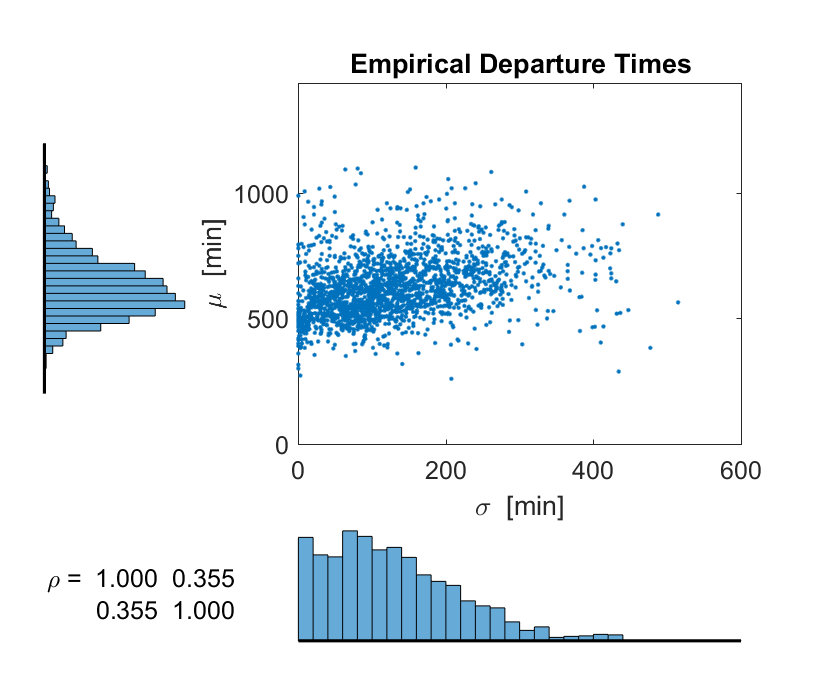
\includegraphics[width=0.48\textwidth,trim={0.4cm 0.4cm 0.4cm 0.4cm}, clip]{figures/mobility/emp_dep.eps}
	}
	\subfloat{
		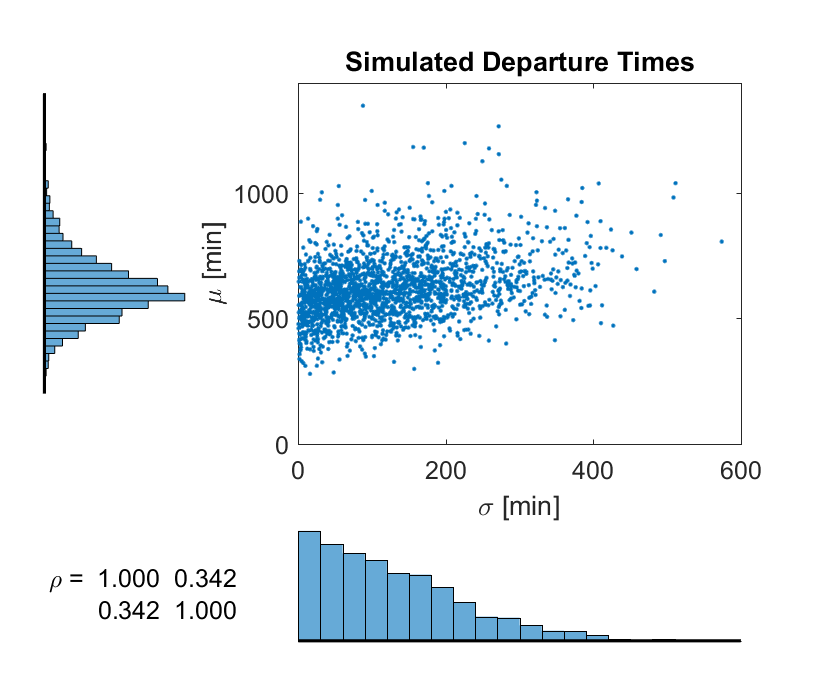
\includegraphics[width=0.48\textwidth,trim={0.4cm 0.4cm 0.4cm 0.4cm}, clip]{figures/mobility/sim_dep.eps}
	}
	\hfill
	\subfloat{
		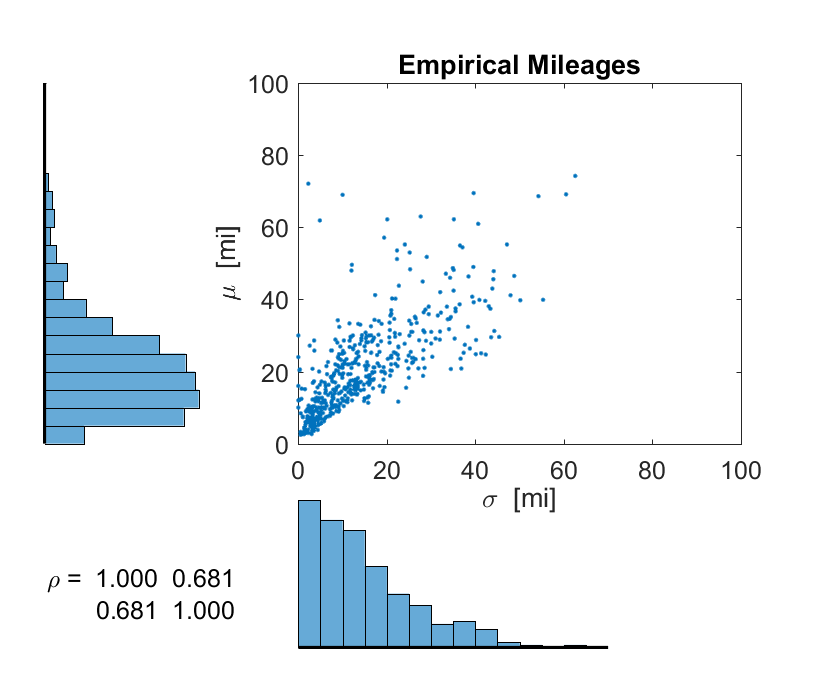
\includegraphics[width=0.48\textwidth,trim={0.4cm 0.4cm 0.4cm 0.4cm}, clip]{figures/mobility/emp_mil.eps}
	}
	\subfloat{
		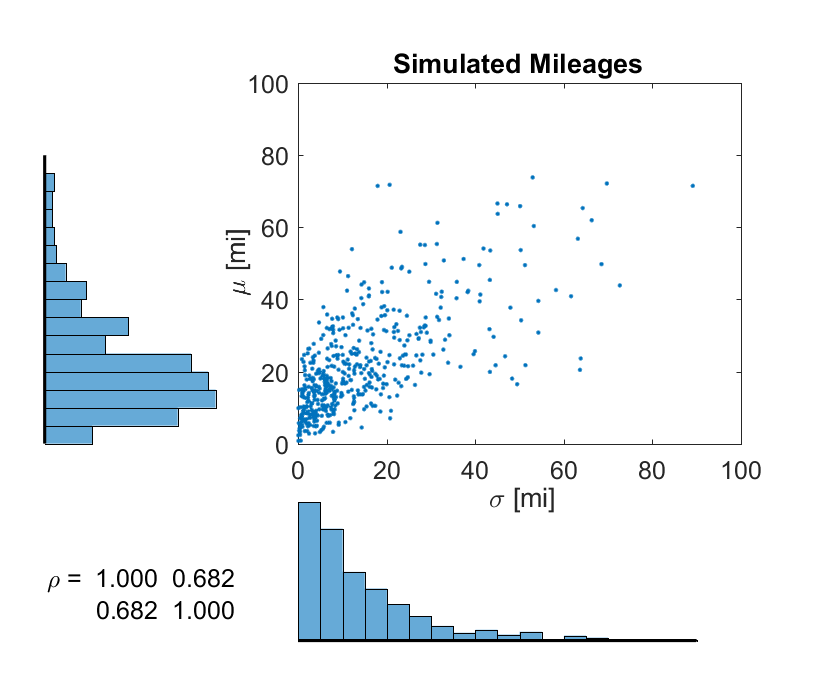
\includegraphics[width=0.48\textwidth,trim={0.4cm 0.4cm 0.4cm 0.4cm}, clip]{figures/mobility/sim_mil.eps}	
	}
	\caption{Correlation of ($\mu$,$\sigma$)-tuples in empirical and simulated driving patterns}
	\label{fig:simmil}
\end{figure}

\newpage
The validity of this approach is investigated by simulating a set of tuples with the size of the empirical data set as presented in the right column of \Autoref{fig:simmil}. The resemblance of empirical and simulated profiles is distinct and supported by similar correlation coefficients of $r=0.682$ for simulated mileages and $r=0.342$ for simulated departure times.

\subsection{Modelling User Behaviour}
\label{sec:mub}

Many studies use empirical or fitted distributions of daily mileage, arrival and departure times for a stochastic scenario generation \cite{Budenbender,Flath2013, Schuller2013, Wu2013,Contreras-Ocana2016, Guo2016, Peppanen2014, Li2014, Salah2016, Richstein2012, Garttner2016c}. Typically, after randomly assigning these parameters to households, they are regarded immutable. A representation of uncertainty involved for each user based on empirical data is, however, less widespread. The acquired knowledge from the preceding sections enables both, stochastic scenario generation and representation of operational uncertainty.

\subsubsection*{Scenario Generation}

The parameters shaping the mobility behaviour of EV owners are generated through realisations of their respective distribution functions and iteratively assigned to households in the test network. The small sample size of days at each household of the survey on which the analysis is based -- peaking at 14 days -- permits no distribution assumption other than the normal distribution $\mathcal{N}(\mu,\sigma)$ for the troika of $(\mu,\sigma)$-tuples defining daily mileage $\tilde{\delta}_{mil}$, arrival time $\tilde{\tau}_{arr}$ and departure time $\tilde{\tau}_{dep}$:

% maximum likelihood: by default forecast is mu as expectation value of normal distribution

\begin{subequations}
	\begin{equation}
		\tilde{\delta}_{mil} \sim \mathcal{N}(\mu_{mil},\sigma_{mil}) \qquad \text{and} \qquad \hat{\delta}_{mil} = \mathbb{E}[\tilde{\delta}_{mil}]= \mu_{mil}
	\end{equation}
	\begin{equation}
		\tilde{\tau}_{arr} \sim \mathcal{N}(\mu_{arr},\sigma_{arr}) \qquad \text{and} \qquad \hat{\tau}_{arr} = \mathbb{E}[\tilde{\tau}_{arr}] = \mu_{arr}
	\end{equation}
	\begin{equation}
		\tilde{\tau}_{dep} \sim \mathcal{N}(\mu_{dep},\sigma_{dep}) \qquad \text{and} \qquad \hat{\tau}_{dep} = \mathbb{E}[\tilde{\tau}_{dep}] = \mu_{dep}
	\end{equation}
\end{subequations}

Simulation under uncertainty will treat $\hat{\delta}_{mil}$, $\hat{\tau}_{arr}$, and $\hat{\tau}_{dep}$ as forecasts and use a realisation of the random variables $\tilde{\delta}_{mil}$, $\tilde{\tau}_{arr}$, and $\tilde{\tau}_{dep}$ to emulate a deviation from predicted parameters.


\subsubsection*{EV Charging Demand}

% tranlate daily mileage to energy consumption / charging demand

Due to the one-to-one correspondence of daily mileage and EV battery discharge linked by the consumption $\zeta = 0.17$ kWh/km and the conversion factor 1.609 km/mi, the battery state of charge upon arrival $\tilde{B}^{arr}$ also follows a normal distribution \cite{Flath2013}. Assuming a full battery at the beginning of the day with a charging level $B_{max} = 30$ kWh and the user does not charge anywhere but at home overnight

\begin{equation}
	\tilde{B}^{arr} = B_{max} - 1.609 \cdot \zeta \cdot \tilde{\delta}_{mil} \qquad \text{and} \qquad \hat{B}^{arr} = B_{max} - 1.609 \cdot \zeta \cdot \hat{\delta}_{mil}.
\end{equation}

If no vehicle belongs to a household, $\tilde{B}^{arr} = \hat{B}^{arr} = {B}^{arr} = B_{max} = 30$ kWh.

\subsubsection*{EV Availability}

The availability of an electric vehicle $\tilde{\alpha}^{EV}\in \mathbb{B}^T$ throughout the optimisation horizon $T=96$ is determined by $\tilde{\tau}_{arr}$, $\tilde{\tau}_{dep}$ and their conversion to time slots $t\in T$:

\begin{equation}
	\tilde{\alpha}^{EV}_t =
	\begin{cases}
	1 & \text{if } \left\lfloor \max \left(0,\; \frac{\tilde{\tau}_{arr}\,-\,\tau_{init}}{\Delta t \cdot 60}\right) \right\rfloor \leq t < \left\lfloor \min \left(T,\; T + \frac{\tilde{\tau}_{dep}\,-\,\tau_{init}}{\Delta t \cdot 60}\right) \right\rfloor\\
	0 & \text{else} 
	\end{cases} \qquad \forall t \in T
\end{equation}

where $\tau_{init} = 660$ min is the time of the day in minutes after midnight at which the optimisation routine starts and $\Delta t$ denotes the granularity. Note that if $\tilde{\tau}_{arr}>\tilde{\tau}_{dep}$ the electric vehicle did not return that night and will not be available for charging at all. The expected availability $\hat{\alpha}^{EV}$ is defined analogously. If no vehicle belongs to a household, $\tilde{\alpha}^{EV}_t = \hat{\alpha}^{EV}_t = {\alpha}^{EV}_t = 0$.

% availability: build availability probabilities 

The probability $\mathbb{P}_t(\alpha^{EV}=1)$ that a vehicle is available in time slot $t$ is calculated using the CDF of the tabulated standard normal distribution $\Phi$ involving the conversion of time slots $t\in T$ to minutes after midnight.

\begin{equation}
\begin{split}
	\mathbb{P}_t\left(\alpha^{EV}=1\right) = \min &\overbrace{\left\{\Phi\left(\frac{ (t \cdot \Delta t \cdot 60 + \tau_{init})-\mu_{arr}}{\sigma_{arr}}\right)\right.}^{\text{probability that vehicle has arrived}},\;\\
& \:\:\,\underbrace{\left.\Phi\left(\frac{ (t \cdot \Delta t \cdot 60 + \tau_{init} - T\cdot \Delta t \cdot 60)-\mu_{dep}}{\sigma_{dep}}\right) \;\right\}}_{\text{probability that vehicle has departed}} \qquad \forall t \in T
\end{split}
\end{equation}

The obtained time series is expedient for the mitigation of availability uncertainty in \mbox{\Autoref{sec:av_unc}}. Exemplary availability probability curves, as well as an average availability probability curve of 55 vehicles, are illustrated in \Autoref{fig:ex_av}. Clearly, the availability of an EV is most likely in the early morning hours and as required reduces towards noon.

% something about average parking duration... 17.5 hours seems so long!

\begin{figure}[b]
	\centering
	\subfloat{
		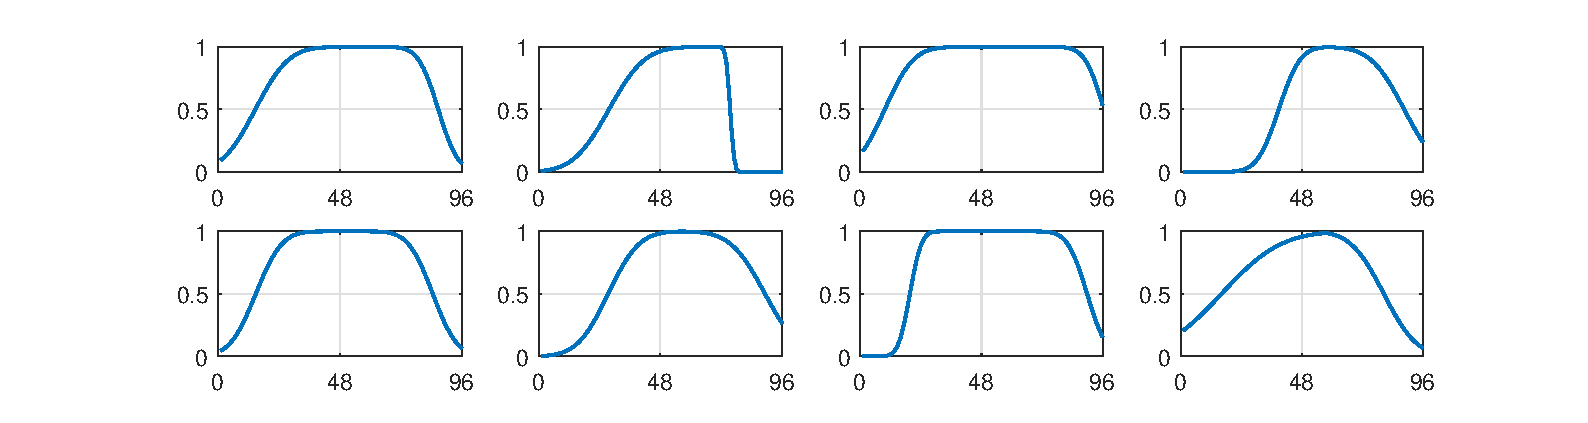
\includegraphics[width=\textwidth,trim={1.5cm 0cm 1.5cm 0cm}, clip]{figures/availability/ex_av.eps}
	
	}
	\vspace{-.5cm}
	\hfill
	\subfloat{
		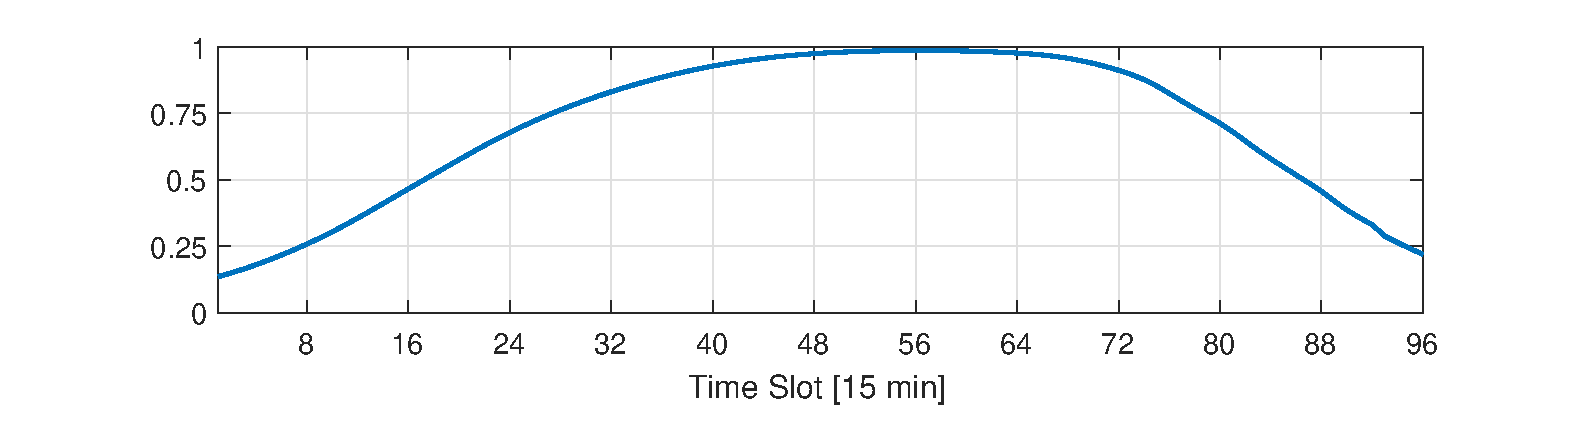
\includegraphics[width=\textwidth,trim={1.5cm 0cm 1.5cm 0cm}, clip]{figures/availability/av_av.eps}
	}
	\caption{Illustration of availability probabilities on an individual (top) or aggregate level (bottom)}
	\label{fig:ex_av}
\end{figure}

\section{Electricity Prices}
\label{sec:ep}

% dynamic tariffs

Dynamically adjusted, time-varying electricity prices as an incentive for stimulating demand-side management are uncommon at the consumer level. Most energy providers offer their customers single or dual rate tariffs, where the latter normally offers a lower price during off-peak periods at night in exchange for a higher price during on-peak hours. 

% support

Support for the integration of intermittent generation by DR or DSM is assumed to be incentivised via wholesale electricity prices. Due to the merit-order effect, the wholesale electricity prices may be used as a proxy for the network state \cite{Kirschen2004}. While low prices indicate low demand or a high share of renewable energy generation and call for an increase in demand, high prices signal peak demand coupled with low renewable generation and urge for a deferral of power demand.

Consequently, the rationale for scheduling approaches seeking to relief network strain and expedite the integration of renewables is to shift deferrable loads to periods with low prices.

\subsection{Modelling}

% data source and illustration, justify choice

To reflect UK power market characteristics, the model for price time series is based on the reference price data (RPD) indices for the EPEX SPOT UK\footnote{formerly APX Power UK / UKPX; first independent power exchange in the UK operating since 2001} energy exchange market, providing a volume-weighted reference price for each half-hourly settlement period. A pool of the 1,000 most recent price profiles is stored from which the stochastic scenario generation picks randomly. \Autoref{fig:var_price} illustrates the diversity of stored price profiles and underlines the tendencies for lower prices at night and price peak during peak demand. Noteworthily, at night outliers below the median dominate while early evening hours exhibit significant outliers above the median concerning both, frequency and magnitude.

\begin{figure}[tp]
	\centering
	\subfloat[Boxplots of stored price profiles]{
		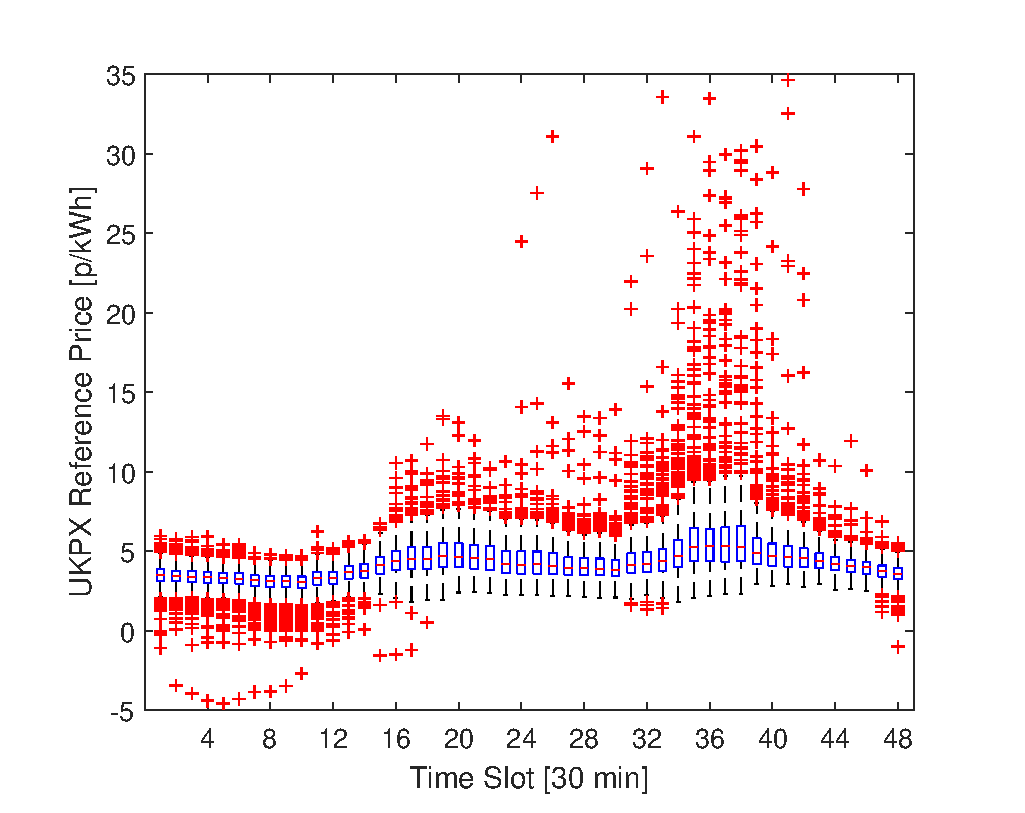
\includegraphics[width=0.48\textwidth]{figures/prices/boxplots_prices.eps}
		\label{fig:pricebox}
	}
	\hfill
	\subfloat[Exemplary price time series (p/kWh)]{
		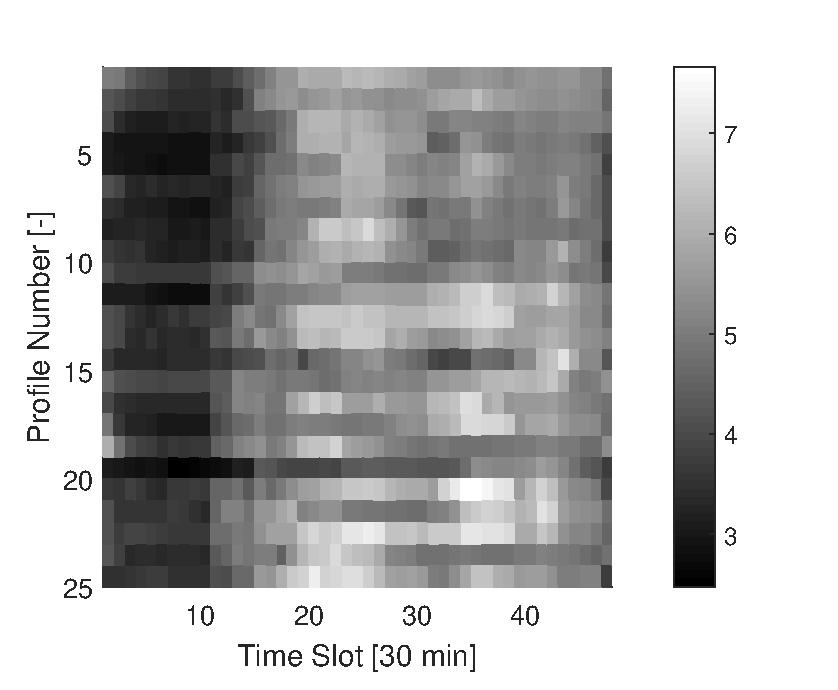
\includegraphics[width=0.48\textwidth]{figures/prices/exemplary_prices.eps}
		\label{fig:exampleprice}
	}
	\caption{Illustration of the variety in price profiles}
	\label{fig:var_price}
\end{figure}

% accessibility - adaptations

In order to unfold the control effect of time-variable pricing, accessibility to customers is essential. This is provided by the aggregator participating in the wholesale market on behalf of the economic interest of its customers. The EPEX SPOT market, however, neither includes license and transmission fees nor taxes, which the aggregator undoubtedly would be charged for selling electricity and pass these costs on. Such charges and fees are mostly constant. The problem with constant charges and fees is that they distort the characteristics of the market price and reduce the signal function for DSM \cite{Jansen2015}. The price of generation and supply is only a fraction of the final electricity price. While static surcharges preserve the ranking of the original price signal and are therefore inconsequential for price-based scheduling approaches, it limits the potential savings of charging coordination. One approach to turn the premiums from a barrier into a driver of demand-side management is to couple the grid charges to the flexible price signal using a multiplicative factor; equivalent to variable fees or taxes. This way the absolute difference of prices is increased and the price signal is amplified. Hence, control agents are further nudged to act market-compliantly through corporate or government incentives \cite{Jansen2015}. 

To simulate the price signal with both variable and static surcharges that on average corresponds to the average retail electricity price of UK single-rate tariffs, the expected price profile is spread around its mean

\begin{equation}
\bar{\pi} = \frac{1}{48}\sum_{t=1}^{48}\hat{\pi}^{EPEX}_t
\end{equation}

by the factor $s=5$ and a constant price addition of $q = 14$ p/kWh is added

\begin{equation}
\hat{\pi}_t = \left(\hat{\pi}^{EPEX}_t-\bar{\pi}\right) \cdot s + \bar{\pi} + q \qquad \forall t \in \{1,\dots,48\}
\end{equation}

to yield the price profile $\hat{\pi}= \left(\hat{\pi}_1,\dots,\hat{\pi}_{48}\right)\in \mathbb{R}^{48}$.

% market power of EV aggregators

\newpage
For simplicity, the influence of additional EV loads on electricity prices is disregarded, and aggregators are not significant enough to exert any market power; i.e.\ all aggregators act as price-takers on the wholesale market \cite{Balram2014, GonzalezVaya2015, Hu2016, Koch2012, Rotering2011}. Moreover, to add variety to the model, the price profiles may be used as a representation of day-ahead or intraday spot market prices depending on the chosen scenario.

% locational marginal prices?

% technical adaptation

To match the number of time intervals of the optimisation routine, the price time series $\hat{\pi}$ is expanded such that for a 24-hour optimisation at 15-minute intervals the price profile becomes

\begin{equation}
\hat{\pi}' = \left(\hat{\pi}_1,\hat{\pi}_1,\dots,\hat{\pi}_{48},\hat{\pi}_{48}\right) \in \mathbb{R}^{96}
\end{equation}

This eschews interpolation and preserves the half-hourly interval of price changes.

\subsection{Uncertainty Representation}
\label{sec:pr_unc}

% general model

The uncertain price profile $\tilde{\pi}\in \mathbb{R}^{48}$ is modelled by a sequence of factors $\kappa \in \mathbb{R}^{48}$ describing the severity of price uncertainty of a time slot as the standard deviation of the forecasted prices $\hat{\pi}$ and a sequence of Gaussian noise $\xi\in \mathbb{R}^{48}$ where $\xi_t\sim \mathcal{N}(0,1)$, such that

\begin{equation}
\tilde{\pi}_t = \hat{\pi}_t + \kappa_t \cdot \xi_t
\end{equation}

and $\tilde{\pi}_t\sim \mathcal{N}\left(\hat{\pi}_t, \kappa_t\right)$. Because the price deviations are likely to be serially correlated in time \cite{Wu2010}, independent Gaussian white noise is unsuitable for the error sequence $\xi$. So-called red noise considers the lag-1 autocorrelation $r$ between two successive elements, and better reflects the dependence of forecast errors in consecutive time steps \cite{Bretherton2014}. A sequence of red noise is generated from a $\mathcal{N}(0,1)$ white noise sequence $\omega\in \mathbb{R}^{48}$ by setting

\begin{subequations}
	\begin{equation}
	\xi_1 = \omega_1
	\end{equation}
	\begin{equation}
	\xi_{t+1} = r\cdot \xi_t + \sqrt{1-r^2} \cdot \omega_{t+1} \qquad \text{for } t > 1.
	\end{equation}
\end{subequations}

Thereby, a strong lag-1 correlation coefficient $r=0.7$ of $\xi_{t}$ and $\xi_{t+1}$ is achieved while maintaining that $\xi_{t}$ follows $\mathcal{N}(0,1)$ \cite{Bretherton2014}. 

% kappa
\newpage
Using the sequence $\kappa$ to define the standard deviation of uncertainty relies on the assumption that a statement not only about the range but also about probability distribution of errors can be obtained from price forecasting mechanisms \cite{Niimura2006,Weron2014a}. For the model, the factor $\kappa_t$ consists of three distinct terms:

\begin{equation}
\kappa_t \;=\; 0.5 \;+\; \frac{|\xi_t|}{4} \;+\; \frac{\left|\hat{\pi}_t-(\bar{\pi}+q)\right|}{\max\left\{\,\left|\hat{\pi}_t-(\bar{\pi}+q)\right| ;\; t \in \{1,\dots,48\}\,\right\} }
\end{equation}

The first summand is the minimum standard deviation of any forecast, the second summand introduces a minor red noise error term to distort the ranking of the simulated price profile compared to its projections, and the third summand normalises the deviation of the price forecast from its mean. This reasonably assumes that price extremes tend to be burdened with particular uncertainty compared to prices closer to the average due to peak demand in one case and an expected high share of intermittent generation in the other. The term weightings were chosen arbitrarily and may be adapted to suit different assumptions about price uncertainty. Approximating the maximum of $\xi_t$ by three standard deviations and noting that the third term lies in the interval [0,1], this configuration maintains $\kappa_t$ in a range between 0.5 and 2.25 p/kWh, which results in reasonable error bands as illustrated in \Autoref{fig:priceuncertainty} \cite{OConnell2014}.
 
\begin{figure}[tp] % TODO update!
	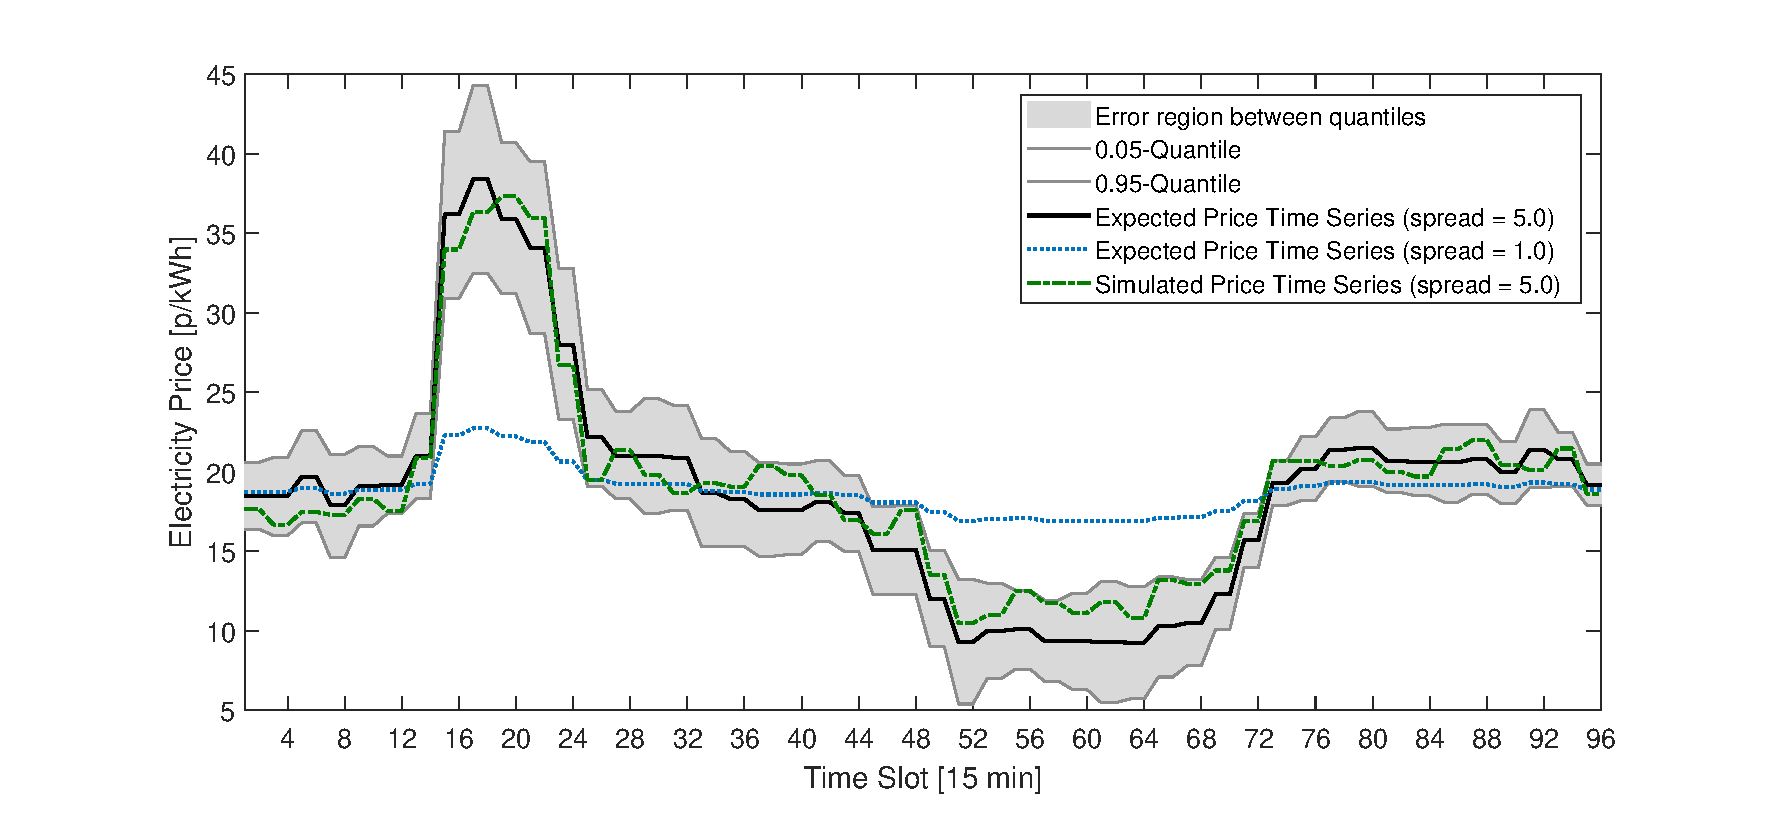
\includegraphics[width=\textwidth,trim={2cm 0cm 2cm 0cm},clip]{figures/prices/price_uncertainty.eps}
	\caption{Exemplary illustration of uncertainty in price time series}
	\label{fig:priceuncertainty}
\end{figure}